\documentclass{ws-p8-50x6-00}
%\documentclass[12pt]{article}
%\pagestyle{empty}

%\makeatletter

%%%%%%%%%%%%%%%%%%%%%%%%%%%%%% User specified LaTeX commands.
\usepackage[dvips]{graphics}
\usepackage{color}
%\usepackage{mac}
%\usepackage{times}
%\usepackage[T1]{fontenc}
%\usepackage{jasa}
%\setlength {\textwidth} {11cm} \setlength {\oddsidemargin} {5 mm}
%\setlength {\textheight} {16cm} \setlength {\topmargin} {0 mm}

%\pagestyle{myheadings}
%\pagestyle{empty}
%\pagefooter{\it SENDI} {JULY 1998} {MECH of HEARING}

\newcommand{\newblock}{}
\newcommand{\Marginpar}[1]{\marginpar{\tiny\setlength{\baselineskip}{.1em}#1}}
\newcommand{\commentX}[1]{}% like this
\newcommand{\comment}[1]{#1}%to remove some stuff remove #1
\newcommand{\bibpath}{/home/jba/doc/bib}
\newcommand{\Fig}[1]{Fig.~\ref{fig:#1}}
\newcommand{\Eq}[1]{Eq.~\ref{eq:#1}}
\newcommand{\Tab}[1]{Table~\ref{tab:#1}}
%\newcommand{\be}{\begin{equation}}
%\newcommand{\ee}{\end{equation}}
\newcommand{\bc}{\begin{center}}
\newcommand{\ec}{\end{center}}
\newcommand{\blue}{\color{blue}}
\newcommand{\red}{\color{red}}
\newcommand{\green}{\color{green}}
\newcommand{\black}{\color{black}}
\newcommand{\magenta}{\color{magenta}}
\newcommand{\cyan}{\color{cyan}}         
\newcommand{\paragraph}[1]{{\bf #1}}
%\makeatother

%\nopagenumbers
\begin{document}

\title{
IS TECTORIAL MEMBRANE FILTERING REQUIRED TO EXPLAIN TWO TONE
	SUPPRESSION AND THE UPWARD SPREAD OF MASKING?
}

\author{Jont B. Allen \& Deep Sen}
\address{AT\&T Labs--Research, Florham Park NJ 07932}
%\date{April 20, 1999}
\maketitle
%\setlength{\baselineskip}{1.1em}
\setlength{\baselineskip}{11pt}

In this paper we would like to make three key points. \emph{First}, neural two
tone suppression (2TS), by low frequency suppressors on high frequency probes,
and the upward spread of masking (USM) are alternate measures of the
same nonlinear cochlear mechanism. The two have similar (i.e., essentially equal)
thresholds and growth rates.
\emph{Second}, the thresholds of neural 2TS, and of the USM, as a function of the
probe frequency, are nearly independent of frequency, and are close to 65 dB SPL.
\emph{Third}, we discuss and model the \emph{level dependence} of 2TS and the USM,
which experimentally has previously been found to be about 2.4 dB/dB in both cat
and human.

Regarding the \emph{first} point: 
%The low frequency tone intensity required to suppress the response of a
%high frequency probe on the basilar membrane (BM-2TS) requires 10 to 20 dB
%greater response at the high frequency place, than probe's BM response.
The dB difference in BM displacement response between a high frequency probe,
and a low frequency threshold suppressor, at the probes place, is 10 to 20 dB
\cite{Ruggero92a,Cooper96b,Geisler97a}.
%This is in contrast to the 0 dB difference in the threshold intensity for
%neural 2TS and neural excitation thresholds.
The BM observations are therefore \emph{in basic disagreement} with corresponding
neural and psychophysical data, which have \emph{similar} thresholds for excitation
and 2TS \cite{Fahey85}.

Regarding the \emph{second} point: When corrected for the middle ear response, the
frequency response slope (i.e., in dB/octave) of the low frequency (basal) portion
of the basilar membrane displacement has a slope of about 9 dB/oct, while the neural
threshold response has a slope close to 0 dB/oct (i.e., less than 1 dB/oct).
This shallow (near zero) basal neural threshold slope shows up as
``tails'' of neural tuning curves.
By transforming neural frequency tuning curves from frequency to place, it is
possible to refine and quantify our understanding of this discrepancy.
This difference in slope is \emph{in fundamental conflict}.

Regarding the \emph{third} point, the 2.4 dB/dB slope implies that, in the
basal ``shallow'' tail, the excitatory response of a low frequency suppressor
(masker) tone ``turns down'' the gain of the probe at a rate of 1.4
dB/dB, re the suppressor (masker) level.
We presume this suppression comes from an outer hair cell (OHC) controlled
gain.  We argue that a level dependent BM stiffness must act as the nonlinear
BM control parameter.

\begin{figure}[ht]
\begin{minipage}[b]{2.75in}
 \centering
	\resizebox{ \textwidth }{!}{ \includegraphics{figs/eplftc.eps} }
\end{minipage}
\hfill
\parbox[b]{1.75in}{
\caption{ \small \setlength{\baselineskip}{.1em}
Shown here are a family of cat neural tuning curves, provided by Delgutte
and Liberman of Eaton Peabody Laboratory, Boston. These frequency tuning
curves were transformed into excitation patterns using the cochlear map of
\Fig{cmap}.
\label{fig:eplftc}
	}}
\end{figure}

\paragraph{Tuning curve tails:}
As may be seen for the 6 kHz neuron in \Fig{eplftc}, the low frequency tails
of high CF threshold neural frequency tuning curves (in the cat)
are typically bowl shaped functions of frequency, largely determined by
the middle ear pressure transfer function ($P_{sv}/P_{ec}$).
For example, in Figure 18c of Allen (1983), \nocite{Allen83a} after
normalizing by the cochlear microphonic to remove the effect of the
middle ear transfer function, the average neural response slope between
0.3-2.0 kHz was found to be 0 dB/oct, $\pm$ 5 dB/oct.
\emph{In sharp contrast}, the displacement of the basilar membrane in this same
basal region is approximately 9 dB/oct, as shown in the following analysis
[see also Allen, 1979]. \nocite{Allen79a,Allen83a}

\begin{figure}[ht]
\begin{minipage}{1.75in}
\resizebox{ \textwidth }{!}{
%\centering
 \includegraphics{figs/cmap.eps} } 
\end{minipage}
\hfill
\raisebox{0.25cm}{
\begin{minipage}{2.5in}
\caption{ \small \setlength{\baselineskip}{.1em}
Plot of the cat cochlear map. The slope of 3 mm/oct was established
by Liberman by direct measurement. The cochlear map may be used to
transform a family of frequency tuning curves into place curves, providing
us with estimates of the neural excitation pattern slopes.  }
\label{fig:cmap}
\end{minipage}
}
\end{figure}

By transforming from frequency to place \cite{Allen90b}, via the \emph{cochlear
frequency to place map} shown in \Fig{cmap}, one may find the threshold neural
place response for a single tone, thereby removing the effect of the middle ear.
For example, in the cat,
where the slope of the cochlear map is 3 mm/oct \cite{Liberman82},
a mechanical [i.e., the BM displacement/scala pressure at the stapes]
slope of 9 dB/oct transforms to 3 dB/mm.
As shown in \Fig{ep1} and \Tab{slopes}, for CFs between 0.25
and 2.0 kHz, this transformation results in \emph{threshold neural place
tuning curves} having basal tail response slopes between 0.3-1.3 dB/mm
\cite{Allen99d}.

\begin{table}[htb]
\begin{minipage}[c]{2in}
        \begin{center}
\begin{tabular}{c|ccc} \hline \hline
CF & $S_1$ & $S_2$ & $S_3$ \\ \hline
{\it kHz} &  & {\it SLOPE$^{\blue *}$ (dB/mm)} & \\ \hline 
5.0 & {\blue **} &   32.7 &  -66.1  \\
4.0 & {\blue **} &   26.3 &  -69.3  \\
2.0 & {\blue  1.3} &   15.2 &  -34.5  \\
1.0 & {\blue  1.2} &   17.4 &  -25.6  \\
0.5 & {\blue  0.3} &   14.8 &  -34.5  \\
0.25 &{\blue  0.3} &   17.1 &  -11.0  \\ \hline
\end{tabular}
        \end{center}
\end{minipage}
\hfill
\begin{minipage}[c]{2in}
\caption{ \small \setlength{\baselineskip}{.1em}
The definition of $S_1$, $S_2$, and $S_3$ are given in
\Fig{ep1}, and are shown as dashed lines superimposed on the neural responses.
{\ $^{\blue *}$Mult by 3 mm/oct to convert to dB/oct}
{\ $^{\red **}$For the CFs at 4 and 5 kHz the data are too limited to make
convincing estimates of $S_1$. Since the effect of the middle ear
is much smaller at these frequencies, one may directly confirm the shallow tail
with respect to frequency, without the frequency to place transformation.}
\label{tab:slopes}
}
\end{minipage}
\end{table}

\begin{figure}[ht]
\begin{minipage}[c]{3.5in}
	\begin{center}
%This figure was made using ~/doc/talks/aro.99/Tail/figs/eps2gif (-r150)
% to generated gif file ep.gif. Then I used /papers/Sendi.99/figs/ep1.fig
\resizebox{ \textwidth }{!}{ 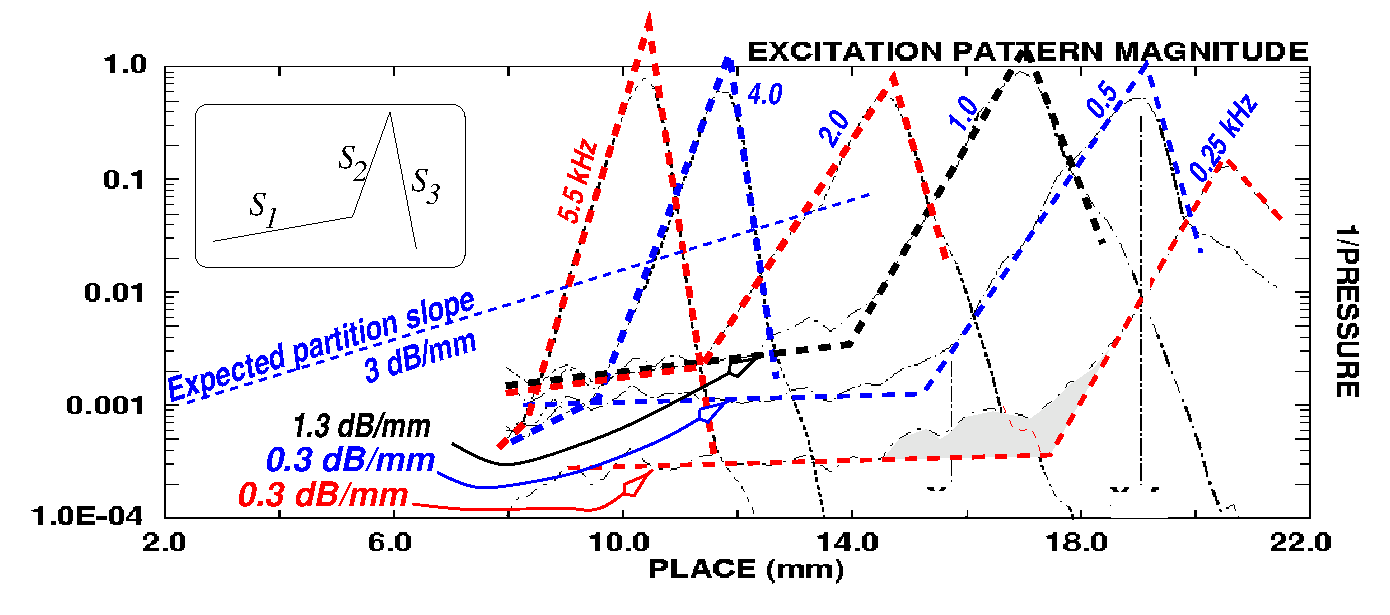
\includegraphics{figs/ep1.eps} } 
	\end{center}
\end{minipage}
\hfill
\raisebox{0.25cm}{
\begin{minipage}[c]{1in}
\caption{ \small \setlength{\baselineskip}{.1em}
Shown here are the resulting excitation patterns derived from the
data of Figures~\ref{fig:eplftc} and \ref{fig:cmap}.
Straight lines have been placed visually on the curves having slopes
as indicated.
\label{fig:ep1} }
\end{minipage}
}
\end{figure}

\paragraph{USM and neural 2TS thresholds.}
The frequency, spatial, and magnitude dependence of these
basal (tail) threshold responses are consistent with the threshold
characteristics of high frequency probes in neural 2TS
\cite{Delgutte90,Abbas76,Fahey85,Sen99a}
and psychophysical USM experiments \cite{Wegel24}.
Namely, as a high level, low frequency, masker (suppressor) is raised in level,
the threshold for masking (suppression) of a high frequency probe is coincident with
the threshold excitation at the low frequency probe's place (in the base). Said another
way, when the cilia excitation in the basal tail approaches threshold levels,
the neural, neural 2TS and USM effects are simultaneously at threshold.
In spatial terms, \emph{these three thresholds occur at almost the same acoustic
intensity over the entire basal tail region of the cochlea}, at about 65
dB SPL \cite{Fahey85}.

From estimates of the human threshold of the USM of Wegel and Lane (1924),
\nocite{Wegel24} we estimate a frequency slope of \(\approx\)5 dB/octave for the
basal tail (this estimate is imprecise).  Since the cochlear map slope in human is
5 mm/octave \cite{Greenwood90}, this corresponds to a slope of
%\cite{Greenwood61,Greenwood61b,Greenwood90}, this corresponds to a slope of
\(\approx\)1 dB/mm for the excitation response in the basal turns of
the human cochlea. Low frequency slopes of 2TS from Abbas and Sachs
(1976) and Fahey and Allen (1985) in the cat are less than 1 dB/mm.
\nocite{Abbas76,Fahey85}

Thus in the base of the cochlea, neural tuning curves, USM thresholds,
and neural 2TS thresholds each indicate a broad flat tail region, both for human
and cat.

%\newpage
\paragraph{A theoretical slope estimate.}
In the base, the partition stiffness
is defined as \( K_p(x) \equiv K_p(0)e^{-2ax} \).
Assuming a constant partition mass and a 3mm/octave frequency to place map,
the value of \( a = \ln(2)/3 \) for the cat is roughly 0.231
{\it mm}$^{-1}$.
From the WKB method, the spatial pressure distribution of a tone stimulus
in the base of the cochlea is given by 
\begin{eqnarray}
\frac{P(x,\omega )}{P(0,\omega )}
				& = &
	\sqrt{\frac{Z_c(x)}{Z_c(0)}}\ \ e^{-i\omega \int _{\xi =0}^x d\xi/c(\xi) } \\
				& = &
	e^{-ax/2} \ e^{-i\omega T(x,\omega)},
\end{eqnarray}
where
the local wave speed is \( c(x)=\sqrt{K_p(x)A(x)/\rho } \) and
the local characteristic impedance is \( Z_c(x) = \sqrt{\rho K_p(x)/A(x)} \).
The effective scala area is $A(x)$ and $\rho$ is the scala fluid density.
% From Chris:
% The expression for Zc in the attachment is missing the sqrt, but looks
% good otherwise. And you're right: the more general expression for Zc,
% valid throughout, is $Zc=\sqrt{Zseries*Zshunt}$. The expression
% $\sqrt{\rho K_p(x)/A(x)}$ is only valid in the base at low frequencies.
%  --Chris
Hair cells are known to be displacement detectors (Hudspeth and Corey, 1977).
Above 1 kHz, Dallos has found that inner hair cells (IHC) respond to displacement.
OHCs are believed to follow displacement at all frequencies.

It follows, from Eq.~2 and Hooke's Law
[ i.e., \(P(x,\omega)=K_p(x)D(x,\omega)\) ],
that the magnitude of the BM displacement \( |D(x,\omega)| \) must vary as
\( e^{3ax/2} \). This corresponds to a BM displacement
slope of about \( 20 \log_{10}(e^{3a/2})\) = 3 dB/mm (i.e., 9 dB/oct)
in the basal tail.%
	\footnote{ \setlength{\baselineskip}{0.1em}
	For this calculation we have taken the area constant. Weaver
	measured $A(x)$ for three human cochleas, and two showed a small
	decrease with $x$. Including this decrease would make the BM
	displacement slope larger, \emph{strengthening} the argument presented here.}
This slope is typical of experimental BM transfer functions \cite{Allen83a}.

	\commentX{ %Leave this out--it is a red herring.
The scala area $A(x)$ has been measured by Weaver for three human
cochleae \cite{Weaver49}.  The measurements show some variation in $A(x)$ between the
three cochleae. In one, the area,%
	\footnote{i.e., $S_v S_t/(S_v+S_t)$ }
shows little net systematic variation with $x$. %Ref Shera and Zweig 91
In the other two, the area decreases by about 50\% between 7 and 25 mm.
If we assume (the extreme case) that $A(x) = e^{-bx}$ varies by
2, then $b \approx 20\log_{10}(2)/35$ = 0.172 dB/mm.
This area variation can therefore slightly reduce the longitudinal dB pressure
variation [the net pressure magnitude exponent would be $-(2a-b)/4x$ rather
than $-ax/2$].  The displacement magnitude exponent would be $[2a-(2a-b)/4]x$.
Such a scala area variation would \emph{increase} the discrepancy between basal
partition displacement and neural spatial variation.
If the pressure were constant (an extreme case), the slope would be 4 dB/mm
(12 dB/oct).

Some have argued that $F_{cf}(x) $ varies as $K_p(x)$ rather than $\sqrt{K_p(x)}$.
If this were true, then the slope might be as low as 2 dB/mm. However I think
these arguments are tenuous, and they imply a 6 dB/oct (3 dB/mm) slope, which seems
smaller than observed. 
Thus the 9 dB/oct (3 dB/mm) slope seems both reasonable and conservative.
	}

%\newpage
\paragraph{Neural 2TS and USM thresholds:}
Fahey and Allen (1985) found the pure tone neural tail and basal neural 2TS thresholds
to be 65 dB SPL for low frequency suppressors between 0.8 and 5 kHz. 
Unpublished data extends this published upper frequency limit to 14 kHz.
	\commentX{
In the cat,
low threshold high frequency neurons (e.g., CF's of 6-10 kHz), when driven
by a 1 kHz low frequency tone, have thresholds around 65 dB SPL (\Fig{eplftc}).
From 2TS experiments, the low-frequency suppression threshold is
also close to 65 dB for high frequency probes \cite{Fahey85}.
Thus (in the cat) \emph{the neural excitation and 2TS threshold levels are similar}.
	}

In stark contrast, recent BM 2TS measurements by
 Ruggero \emph{et al.} (1992), \nocite{Ruggero92a}
 Cooper (1996), \nocite{Cooper96b} and
 Geisler and Nuttall (1997), \nocite{Geisler97a}
have shown unequivocally that the neural and BM 2TS thresholds are
\emph{significantly} different (unlike the cat neuron, where they
are the same). For example, Ruggero \emph{et al.} say (page 1096)
	\begin{quote}
\ldots if neural
rate threshold actually corresponds to a constant displacement ($\approx$ 2 nm)
\ldots, then mechanical suppression thresholds would substantially exceed neural
excitation thresholds and would stand in disagreement with findings on neural
rate suppression.
	\end{quote}
Using a 0.1 nm displacement criterion, Cooper found basal excitation
thresholds near 65 dB and 2TS thresholds near 85 dB SPL. 
Cooper says (page 3095)
	\begin{quote}
Indeed, the direct comparisons shown \ldots indicate that most of
the low-frequency mechanical suppression thresholds were between 10 and
20 dB above the iso-displacement tuning curves[,] which corresponded to
``neural thresholds'' at the site's [CF].
	\end{quote}
That is, Cooper's BM results placed the threshold of BM suppression about 1
order of magnitude higher in level than the Fahey and Allen 2TS thresholds,
both in absolute terms, and relative to the 0.1 nm threshold.
The Geisler and Nuttall (1997) study confirms these findings (see their Fig. 2).
A second unequivocal finding of the studies \cite{Cooper96b,Geisler97a} is
that nonlinear suppression is dependent on BM displacement rather than
velocity.

\emph{In summary}, we have highlighted two important differences between
neural and BM experimental data:
	{\it (i)}
As detailed in \Tab{slopes}, there is a discrepancy in the relative slopes
of neural threshold response and BM displacement of between 3 and 10 in the
basal tail (0.3-1 dB/mm vs. 3 dB/mm) \cite{Allen99d}.
	{\it (ii)}
The dB difference in the threshold intensity for neural 2TS and neural excitation
thresholds is close to 0 dB over a wide range of frequencies, but differ by
10 to 20 dB when measured on the BM.
\emph{ We believe these two problems are related.}%
	\footnote{ \setlength{\baselineskip}{0.1em}
	Suppression on the BM has not yet been measured as a function of
	the probe frequency. If the CF is level dependent, as we believe, then this
	would be an important experiment.
	}

\begin{figure}[ht]
\begin{minipage}[c]{3in}
	\begin{center}
\resizebox{ \textwidth }{!}{ 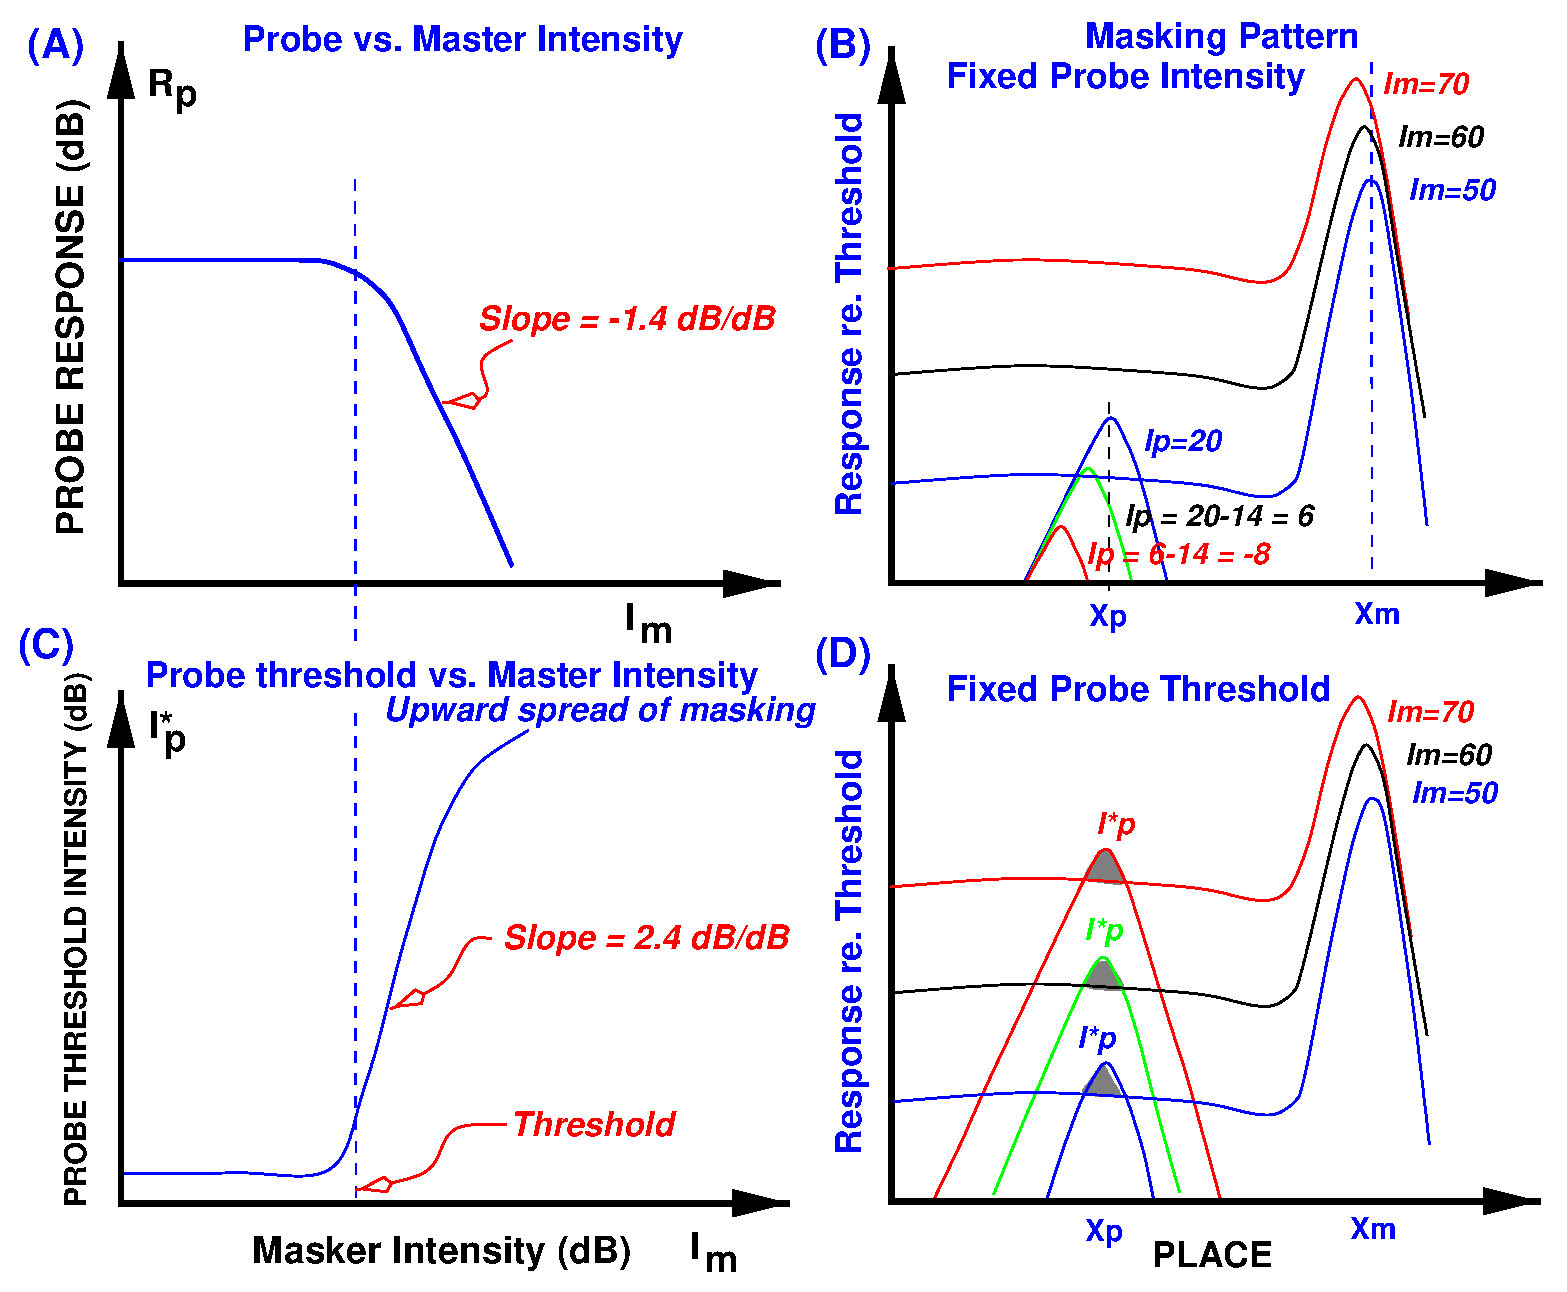
\includegraphics{figs/MaskedGain.eps} } 
	\end{center}
\end{minipage}
\hfill
\raisebox{0.25cm}{
\begin{minipage}[c]{1.5in}
\caption{ \small \setlength{\baselineskip}{.1em}
Panels (A,B) depict (in a cartoon format) what must happen to the
hair cell cilia response of a high frequency probe tone as a low frequency
excitatory suppressor tone is increased in intensity.
(A) depicts the level function for the suppressed response of the probe,
as a function of the suppressor intensity.
Panels (C,D) depict the probe after an adjustment back to its detection
threshold.  (C) shows the level function for the
threshold probe intensity as a function of the suppressor intensity.
\label{fig:MaskedGain}
}
\end{minipage}
} %raisebox
\end{figure}

\paragraph{The slope of 2TS and USM:}
Suppression and USM super-threshold data are exquisitely interesting.
Delgutte (1990) \nocite{Delgutte90} found a 2TS slope of 2.4 dB for every
dB of suppressor level.  We have estimated the same slopes of 2.4 dB/dB from
Wegel and Lane's 1924 USM IO functions (level of a 2-4 kHz probe, at
threshold, as a function of a 400 Hz masker's intensity).%
	\footnote{ \setlength{\baselineskip}{0.1em}
The slopes for the experimental BM data seem to be uncertain.}

We show a summarizing cartoon (\Fig{MaskedGain}) to help explain and summarize
our view of the data. Panels (A,B) depict the response of a fixed probe,
to a low frequency masker, at three masker intensities.
In (B) we depict the IO function of the
probe, with a slope of 1.4 = 2.4 -- 1 dB/dB. The probe must be attenuated
by 1.4 dB for every dB of suppressor (masker) level.
Since the probe (its intensity is fixed) is not returned to threshold,
its slope must be --1.4 dB/dB.
In (C,D) we see the same situation, except
the probe is returned to threshold.
The IO function in this case is 2.4 = 1.4 + 1 dB/dB
since it must overcome the basal linear masker growth.
In summary, as the masker
is increased by 1 dB, the probe is attenuated by 1.4 dB. To return the
probe to threshold, it must be increased by 1.4 dB to overcome the
attenuation, and another 1 dB to overcome the masker level increase,
giving a total of 2.4 dB/dB. What remains unexplained is how the masker
can reduce the gain of the probe in this manner.

\begin{figure}[ht]
\begin{minipage}[c]{2.75in}
	\begin{center}
\resizebox{ \textwidth }{!}{ 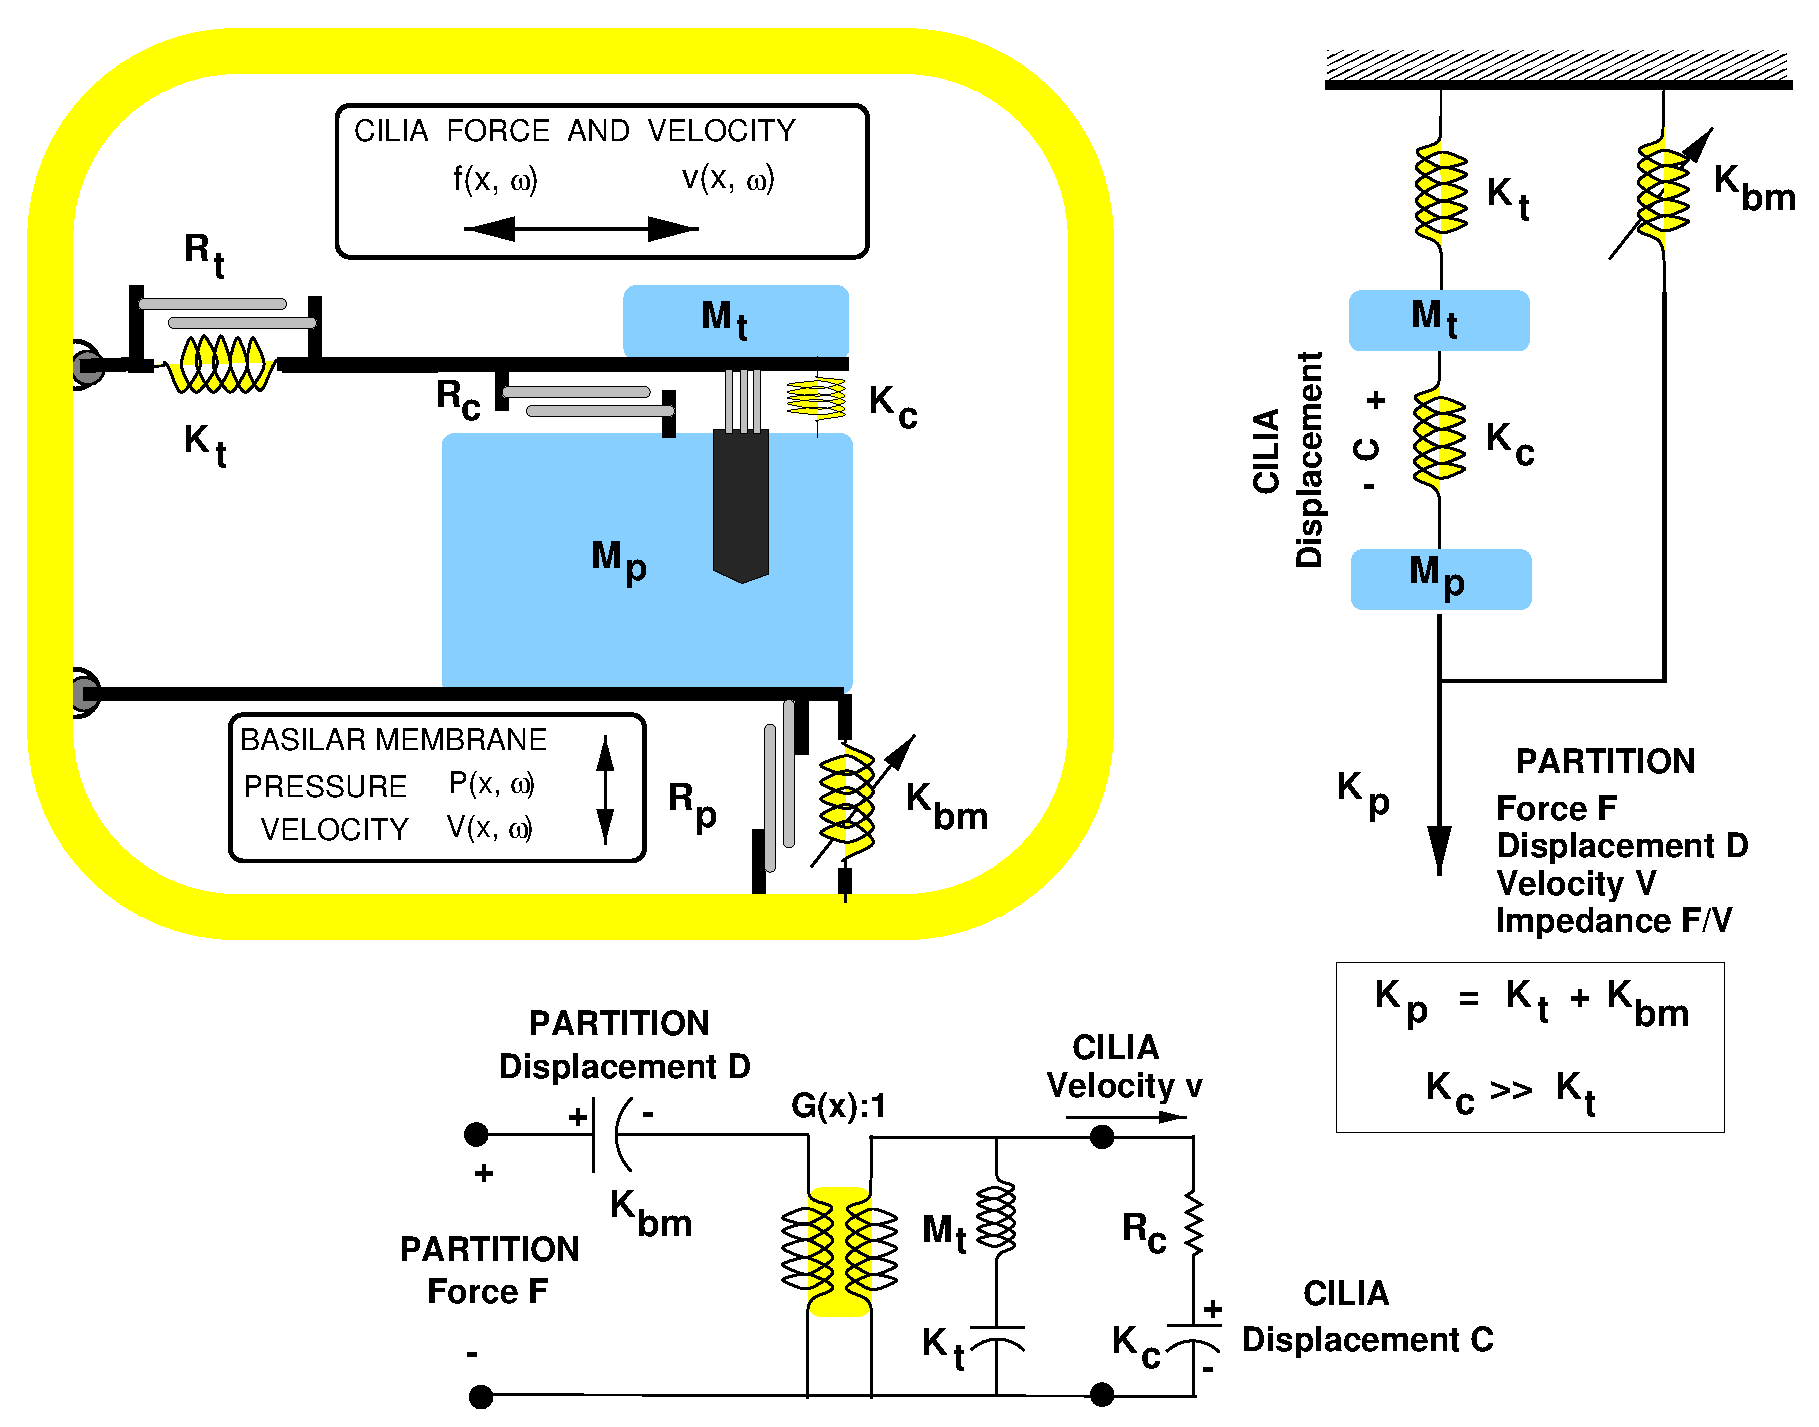
\includegraphics{figs/rectamodel.eps} } 
	\end{center}
\end{minipage}
\hfill
\begin{minipage}[c]{1.25in}
\caption{ \small \setlength{\baselineskip}{.1em}
If the partition stiffness $K_p(x)$ is dominated by the stiffness of the tectorial
membrane $K_t(x)$ at high intensities, and the OHCs induced stiffness (a dynamic
nonlinear component of the stiffness) at low intensities, then a simple model can
satisfy all the required conditions simultaneously.
\label{fig:rectamodel}
}
\end{minipage}
\end{figure}

\paragraph{A robust solution:}
	\commentX{
There might be several possible explanations to the slope and BM suppression
discrepancies.  Perhaps the inner and outer hair cells (OHC) have significantly
different sensitivities, and vary as \( e^{-2ax} \).  However, there is no
evidence for an exponentially varying sensitivity of the hair cells;
if anything, evidence suggests that their sensitivity \emph{increases} as a
function of \( x \), due to the increasing cilia length with place.}
%A more likely solution is that 
We propose that the micromechanics of the tectorial membrane (TM) transforms
the BM displacement slope of 3 dB/mm to a cilia excitation which has almost
constant place dependence ($<$0.3 dB/mm in cat).
From \Fig{rectamodel} it follows that the cilia to BM displacement ratio is
	$H_c \equiv C/D = K_t/(K_c+K_t)$.  
It is required, by the TM model \cite{Allen80}, that
the cilia be much stiffer than the TM ($K_c >> K_t$), thereby attenuating
the cilia response in the base.  Thus $H_c \approx K_t/K_c << 1 $.

If the TM to cilia stiffness ratio $K_t(x)/K_c(x)$ were to vary as
	\( e^{-3ax/2} \)
it would compensate for the \( e^{3ax/2} \) dependence of the BM displacement.
If two springs are in series, and one is much stiffer, the total stiffness is
dominated by the smaller stiffness, namely
	\( K_t K_c/(K_t + K_c) \approx K_t \).
The partition stiffness is therefore $K_p \approx K_t +K_{bm}(C)$.
The second term is the dynamic OHC component of the stiffness which depends
on the cilia displacement $C$, and is approximately equal to $K_t$ in
quiet (i.e., $C=0$), and at very high intensities, or in a dead ear, approaches zero.
This gives us enough equations to determine every element uniquely,
in a manner that is consistent with our requirements.
It follows that the cilia stiffness must be
	\( K_c(x) = K_p(0) e^{-ax/2} \).
The fact that OHC cilia increase in length [from 4 to 6 $\mu$m in the cat] is
qualitatively consistent with this decreasing $K_c(x)$.

Under these conditions,
{\it (1)} the TM stiffness is proportional to
	\( e^{-2ax} \) [i.e., \(K_t \propto K_p(x)\)];
{\it (2)} at high intensities, $K_t(x)$ determines the partition stiffness $K_p(x)$;
{\it (3)} the transduction ``filter'' $H_c(x,f)$ cancels the 3 dB/mm (9 dB/oct)
BM displacement growth giving a cilia response with a close to zero slope. 
Since the partition stiffness is mainly determined by the TM stiffness,
[plus an equal dynamic, nonlinear component due to the OHCs at low intensities
	\( K_{bm}(C) \)],
this choice of parameters naturally accounts for the necessary correlation
in the partition and TM stiffness variation.

We would like to thank Christopher Shera and Paul Fahey for their help.

%\newpage
\begin{small}
\setlength{\baselineskip}{0.9em}
\bibliographystyle{abbrv}
\bibliography{\bibpath/oae,\bibpath/jnd,\bibpath/allen,\bibpath/fletcher,%
\bibpath/loudness,\bibpath/model,\bibpath/books}
\end{small}
\vfill\flushleft {\tiny /doc/papers/Sendhi.99/Paper.tex}

\end{document}
